\documentclass[a4paper]{article}

\usepackage[table]{xcolor}%this has to be the first!!!!!!
\usepackage{fullpage} % Package to use full page
%\usepackage{parskip} % Package to tweak paragraph skipping
\usepackage{tikz} % Package for drawing
\usetikzlibrary{shapes,arrows,matrix,positioning}
\usepackage{amsmath}
\usepackage{indentfirst}
\usepackage{hyperref}
\usepackage{subcaption}
\usepackage{graphics}
\usepackage{graphicx}
\usepackage{minted}
\usepackage{multicol}
%color define
\definecolor{codebg}{RGB}{230,255,253}
\definecolor{function}{RGB}{210,0,26}
\definecolor{para}{RGB}{255,137,137}
\definecolor{output}{RGB}{238,224,201}
\setminted[lexer.py:DiffLexer -x]{mathescape=true,breaklines,bgcolor=codebg,linenos}

\tikzset{
  block/.style = {rectangle, draw, fill=output, text width=6cm, text centered, rounded corners, minimum height=4em},
  line/.style = {draw, -latex'},
}


%function newcommand
\newcommand{\func}[1]{\textbf{\textcolor{function}{#1}}}
\newcommand{\para}[1]{\textbf{\emph{\textcolor{para}{#1}}}}

\usepackage{biblatex}
\addbibresource{bibliography.bib}
\title{bcg.h Documentation}
\author{Haochen(Langford) Huang}
\date{\today}

\begin{document}

\maketitle

\section{Introduction and Background}\label{sec:intro}
\textbf{bcg.h} file contains two functions: \textcolor{red}{\emph{tracer\_fluxes}} and \textcolor{red}{\emph{advection}} whose major purpose is to construct a solver for advective equation:
\begin{equation}
  \frac{\partial \Phi}{\partial t} + ( \mathbf{u} \cdot \nabla)\Phi = 0\label{equ:aim}
\end{equation}
where $\Phi$ is the scalar and $ \mathbf{u}$ is the velocity. The discrete time formulation of Eq.\ref{equ:aim} reads:
\begin{equation}
  \frac{\Phi^{n+1}-\Phi^{n}}{\Delta t} + \mathbf{A}^{n+\frac{1}{2}} = 0 \label{equ:general}
\end{equation}
Where $ \mathbf{A}^{n+ \frac{1}{2}}$ is the abbraviation of advection term in BCG\cite{bell1989second,popinet2003gerris} scheme (and is the reason why the name of this file called 'bcg.h'), and is intergrated within the controled volume
\begin{equation}
  \int_{\Gamma} A^{n+ \frac{1}{2}} = \int_{\Gamma} [( \mathbf{u}\cdot \nabla)\Phi]^{n+ \frac{1}{2}} = \int_{\Gamma} [\nabla\cdot( \mathbf{u} \Phi)]^{n+ \frac{1}{2}} = \int_{\partial \Gamma} ( \mathbf{u}^{n + \frac{1}{2}} \cdot \mathbf{n}) \Phi^{n+ \frac{1}{2}}
\end{equation}
The second step above is achieved by combining divergence free constraints $\nabla\cdot \mathbf{u}=0$ and the $ \mathbf{n}$ represents the normal direction of cell interface. For quadtree or octree cells, the overall caculation turns out to be
\begin{equation}
  \Delta A^{n+ \frac{1}{2}} = \sum_{i=d} u_d^{n+ \frac{1}{2}}\Phi_d^{n + \frac{1}{2}} 
\end{equation}
where $u_d$ is the component of $ \mathbf{u}$ on normal direction of interface, $Delta$ is the length of the cell and $\Phi_d$ is the corresponding value at the interface. Then the critical is how to obtain $\Phi_d^{n + \frac{1}{2}}$. According to \cite{popinet2003gerris}, using Taylor expansion we have
\begin{equation}
  \Phi^{n+ \frac{1}{2}}_d = \Phi^n+ \frac{\Delta}{2} \frac{\partial \Phi^n}{\partial x_d} + \frac{\Delta t}{2} \frac{\partial \Phi^n}{\partial t} + O(\Delta^2,\Delta t^2)
\end{equation}
Replacing $ \frac{\partial \Phi^n}{\partial x_d}$ with Eq.\ref{equ:aim} yielding 
\begin{equation}
  \Phi^{n+ \frac{1}{2}}_d = \Phi^n + [\frac{\Delta}{2}- \frac{\Delta t}{2} \mathbf{u}^n \cdot \mathbf{n}_d] \frac{\partial \Phi^n}{\partial x_d} - \frac{\Delta t}{2} \mathbf{u}^n\cdot \mathbf{n}_e \frac{\partial \Phi^n}{\partial x_e} - \frac{\Delta t}{2} \mathbf{g}^n \label{equ:taylor}
\end{equation}
Subscript $e$ represents direction other than current direction $d$.
Compromise is taken for sake of convenience (maybe) that $ \mathbf{u}^n$ in Eq.\ref{equ:taylor} is repleced by $ \mathbf{u}^{n + \frac{1}{2}}$ so that $ \mathbf{u}^n\cdot \mathbf{n}_d$ can be computed by $u_d^{n + \frac{1}{2}}$. (see Sec.\ref{sec:tracerdetail} for more details).
\section{Functions}

\subsection{\func{tracer\_fluxes}}

\subsubsection{Parameters}
\begin{center}
  \begin{tabular}{|c|c|c|c|c|}
    \hline
    Name & Data type & Status & Option & Representation (before/after)\\[0.5ex]
    \hline\hline
    \para{f} & scalar & unchange & complusory & $\Phi^n$\\
    \hline
    \para{uf} & face vector & unchange & complusory & $u_d^{n+ \frac{1}{2}}$\\
    \hline
    \rowcolor{output} \para{flux} & face vector & \textbf{output} & complusory & $u_d^{n+ \frac{1}{2}}\Phi_d^{n+\frac{1}{2}}$\\
    \hline
    \para{dt} & double & unchange & complusory & $\Delta t$\\
    \hline
    \para{src} & scalar & unchange & complusory & $ \mathbf{g}^n$ \\
    \hline
  \end{tabular}
\end{center}

\subsubsection{Worth Mentioning Details}\label{sec:tracerdetail}
Data of \emph{face vector} type is stored on staggered mesh\cite{harlow1965numerical}. Take \para{uf} as an example, the storage on a 2D cell displays in Fig.\ref{fig:staggered}.
\begin{figure}[H]
     \centering
     \begin{center}
     \begin{tikzpicture}[scale=1]
     \draw (-2,0)--(2,0)--(2,4)--(-2,4)--(-2,0);
     \draw[->] (0,-0.25)--(0,0.75) node[anchor=west]{ $uf_{y}[i]$ };
     \draw[->] (-2.25,2.0)--(-1.25,2.0) node[anchor=west]{ $uf_x[i]$ };
     \draw[->] (0,3.75)--(0,4.75) node[anchor=west]{ $uf_{y}[i+1]$ };
     \draw[->] (1.75,2)--(2.75,2) node[anchor=west]{ $uf_x [i+1]$ };
     \end{tikzpicture}
     \end{center}
     \caption{Staggered mesh.}
     \label{fig:staggered}
\end{figure}
Components are saved in corresponding face with single value. The direction of the component express itself in the feature of the cell face. Therefore, $ \mathbf{u}^{n + \frac{1}{2}} \cdot \mathbf{n}_x$ can simply be $ \frac{1}{2}(uf_x[i]+uf_x[i+1])$.\par
Advection term employs BCG scheme\cite{martin2000cell}, a second order upwinded scheme. It first requires face-centered approximation of velocity $u_d^n,v_e^n(w_f^n)$. Then Eq.\ref{equ:taylor} is adapted to a upwinded scheme
\begin{equation}
  \Phi_d^{n+ \frac{1}{2}}=
    \left \{ 
    \begin{array}{cc}
      \bar{\Phi}^{L,n+ \frac{1}{2}}_d\quad &if\, u_d^n>0,\\
      \bar{\Phi}^{R,n+ \frac{1}{2}}_d\quad &if\, u_d^n<0,\\
      \frac{1}{2}(\bar{\Phi}^{L,n+ \frac{1}{2}}_d+\bar{\Phi}^{R,n+ \frac{1}{2}}_d)\quad &if \,u_d^n=0.
    \end{array}
    \right.
\end{equation}
where
\begin{align}
  \bar{\Phi}^{L,n+ \frac{1}{2}}_d &= \Phi^n[i] + \frac{\Delta}{2}min[1- \frac{\Delta t}{2\Delta}(u_d^n[i]+u_d^n[i+1]),1] \frac{\partial \Phi}{\partial x_d}[i]- \frac{\Delta t}{2} \mathbf{g}^n-flux_e[i]\\
  \bar{\Phi}^{R,n+ \frac{1}{2}}_d &= \Phi^n[i+1] - \frac{\Delta}{2}min[1- \frac{\Delta t}{2\Delta}(u_d^n[i]+u_d^n[i+1]),1]\frac{\partial \Phi}{\partial x_d}[i+1]- \frac{\Delta t}{2} \mathbf{g}^n-flux_e[i+1]
\end{align}
$flux_e$ represents contrubution from direction other than $d$, which also takes upwinded scheme
\begin{equation}
    flux_e = \frac{\Delta t}{2} \mathbf{u}^n\cdot\mathbf{n}_e \frac{\partial \Phi^n}{\partial x_e}=\left \{ 
    \begin{array}{cc}
      \frac{\Delta t}{2\Delta} v_{e}^{trans}(u^n[i,j]-u^n[i,j-1])\quad if\,v_{e}^{trans}>0,\\
      -\frac{\Delta t}{2\Delta} v_e^{trans}(u^n[i,j]-u^n[i,j+1])\quad if\,v_e^{trans}<0.
    \end{array}
    \right.
\end{equation}
where $v_e^{trans} = \frac{1}{2}(v_e^{trans}[i,j]+v_e^{trans}[i,j+1])$
\subsubsection{Program Workflow}
\begin{multicols}{2}
  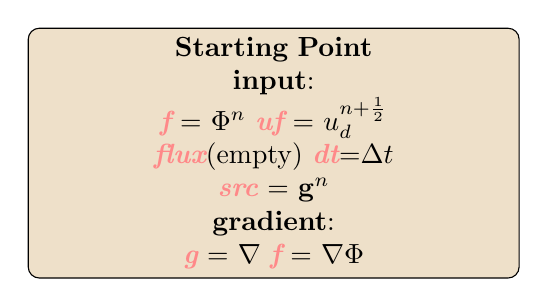
\begin{tikzpicture}
    \node [block](init){
        \textbf{Starting Point}\\
        \textbf{input}: \\
        \para{f} = $\Phi^n$ \para{uf} = $u_d^{n+ \frac{1}{2}}$\\ \para{flux}(empty) \para{dt}=$\Delta t$\\ \para{src} = $ \mathbf{g}^n$\\
        \textbf{gradient}:\\
        \para{g} = $\nabla$ \para{f} = $\nabla \Phi$
      };
  \end{tikzpicture}
 \columnbreak
 \begin{minted}[obeytabs=false,mathescape=true,breaklines]{lexer.py:DiffLexer -x}
void tracer_fluxes (scalar f,
		    face vector uf,
		    face vector flux,
		    double dt,
		    (const) scalar src)
{
  vector g[];
  gradients ({f}, {g});
 \end{minted}
\end{multicols}

\begin{center}
  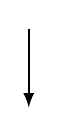
\begin{tikzpicture}
    \draw[-latex,thick](0,0) -- (0,-1); 
  \end{tikzpicture}
\end{center}

\begin{multicols}{2}
  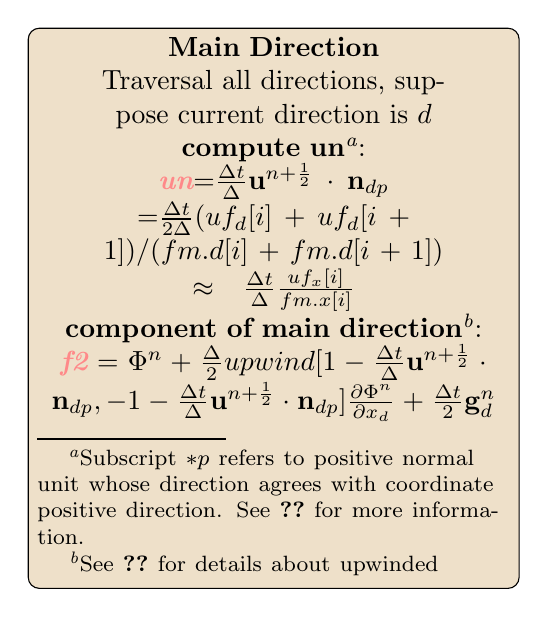
\begin{tikzpicture}
    \node [block](init){
        \textbf{Main Direction}\\
        Traversal all directions, suppose current direction is $d$\\
        \textbf{compute un}\footnote{Subscript $*p$ refers to positive normal unit whose direction agrees with coordinate positive direction. See \ref{sec:direction} for more information.}: \\
        \para{un}=$ \frac{\Delta t}{\Delta}\mathbf{u}^{n+ \frac{1}{2}}\cdot \mathbf{n}_{dp}$\\=$ \frac{\Delta t}{2\Delta}(uf_d[i]+uf_d[i+1])/(fm.d[i]+fm.d[i+1])$\\ $\approx  \frac{\Delta t}{\Delta} \frac{uf_x[i]}{fm.x[i]}$\\
        \textbf{component of main direction}\footnote{See \ref{sec:tracerdetail} for details about upwinded }:\\
        \para{f2} = $\Phi^n + \frac{\Delta}{2}upwind[1- \frac{\Delta t}{\Delta} \mathbf{u}^{n+\frac{1}{2}}\cdot \mathbf{n}_{dp},-1-\frac{\Delta t}{\Delta} \mathbf{u}^{n+\frac{1}{2}}\cdot \mathbf{n}_{dp}] \frac{\partial \Phi^n}{\partial x_d}+\frac{\Delta t}{2}\mathbf{g}_d^n$ 
      };
  \end{tikzpicture}
  \columnbreak
  \begin{minted}[obeytabs=false,mathescape=true,breaklines]{lexer.py:DiffLexer -x}
  foreach_face() {
    double un = dt*uf.x[]/(fm.x[]*Delta + SEPS), s = sign(un);
    int i = -(s + 1.)/2.;
    double f2 = f[i] + (src[] + src[-1])*dt/4. + s*(1. - s*un)*g.x[i]*Delta/2.;
  \end{minted}
\end{multicols}

\begin{center}
  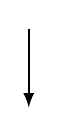
\begin{tikzpicture}
    \draw[-latex,thick](0,0) -- (0,-1); 
  \end{tikzpicture}
\end{center}

\begin{multicols}{2}
  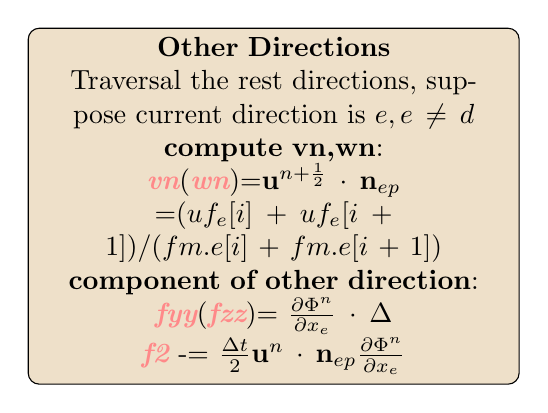
\begin{tikzpicture}
    \node [block](init){
        \textbf{Other Directions}\\
        Traversal the rest directions, suppose current direction is $e,e\neq d$\\
        \textbf{compute vn,wn}: \\
        \para{vn}(\para{wn})=$\mathbf{u}^{n+ \frac{1}{2}}\cdot \mathbf{n}_{ep}$\\=$(uf_e[i]+uf_e[i+1])/(fm.e[i]+fm.e[i+1])$\\
        \textbf{component of other direction}:\\
        \para{fyy}(\para{fzz})= $\frac{\partial \Phi^n}{\partial x_e}\cdot \Delta$\\
        \para{f2} -= $ \frac{\Delta t}{2} \mathbf{u}^n\cdot \mathbf{n}_{ep} \frac{\partial \Phi^n}{\partial x_e}$ 
      };
  \end{tikzpicture}
  \columnbreak
  \begin{minted}[obeytabs=false,mathescape=true,breaklines]{lexer.py:DiffLexer -x}
    #if dimension > 1
    if (fm.y[i] && fm.y[i,1]) {
      double vn = (uf.y[i] + uf.y[i,1])/(fm.y[i] + fm.y[i,1]);
      double fyy = vn < 0. ? f[i,1] - f[i] : f[i] - f[i,-1];
      f2 -= dt*vn*fyy/(2.*Delta);
    }
    #endif
    #if dimension > 2
    if (fm.z[i] && fm.z[i,0,1]) {
      double wn = (uf.z[i] + uf.z[i,0,1])/(fm.z[i] + fm.z[i,0,1]);
      double fzz = wn < 0. ? f[i,0,1] - f[i] : f[i] - f[i,0,-1];
      f2 -= dt*wn*fzz/(2.*Delta);
    }
    #endif
  \end{minted}
\end{multicols}

\begin{center}
  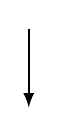
\begin{tikzpicture}
    \draw[-latex,thick](0,0) -- (0,-1); 
  \end{tikzpicture}
\end{center}

\begin{multicols}{2}
  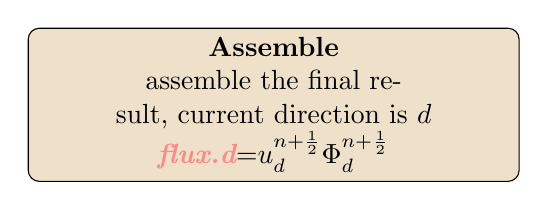
\begin{tikzpicture}
    \node [block](init){
        \textbf{Assemble}\\
        assemble the final result, current direction is $d$\\
        \para{flux.d}=$u_d^{n+ \frac{1}{2}}\Phi_d^{n+ \frac{1}{2}}$
      };
  \end{tikzpicture}
  \columnbreak
  \begin{minted}[obeytabs=false,mathescape=true,breaklines]{lexer.py:DiffLexer -x}
    flux.x[] = f2*uf.x[];
  }
}
  \end{minted}
\end{multicols}

\subsection{\func{advection}}

\subsubsection{Parameters}
\begin{center}
  \begin{tabular}{|c|c|c|c|c|}
    \hline
    Name & Data type & Status & Option & Representation (before/after)\\[0.5ex]
    \hline\hline
    \rowcolor{output} \para{tracers} & scalar* & update & complusory & $\Phi^n$/ $\Phi^n-\Delta t A^{n+ \frac{1}{2}}$\\
    \hline
    \para{u} & face vector & unchange & complusory & $u_d^{n+ \frac{1}{2}}$\\
    \hline
    \para{dt} & double & unchange & complusory & $\Delta t$\\
    \hline
    \para{src} & scalar* & unchange & optional & $ \mathbf{g}^n$ \\
    \hline
  \end{tabular}
\end{center}

\subsubsection{Worth Mentioning Details}\label{sec:direction}
The input of this function (\para{tracers},\para{src}) can be $vector$ type, \emph{e.g.} $ \mathbf{u}$, where components of each direction is deemed as $scalar$ type data then is finally assembled as a $vector$.\par
Aonther thing needs to be concerned is the direction of the normal unity associates with coordinate axis. Positive direction of coordinate remains unchanged will face normal direction varies with respect to current cell. Take Fig.\ref{fig:facenormal} as an example. \begin{figure}[H]
  \centering
    \begin{tikzpicture}[scale=1]
    \draw[->] (-3,0) -- (3,0) node[anchor=north west] {x};%画出x轴并将最后的终结点其命名为x
    \draw[->] (0,-1) -- (0,3) node[anchor=south east] {y};%画出y轴并将最后的终结点其命名为y
    \draw[very thick,red]
        (0,0) -- (0,2.5);%在线段的中间添加标签,并使用fill = white使线条不透过标签
    \draw (-2.5,0) -- (-2.5,2.5)--(2.5,2.5)--(2.5,0);
    \fill [color = red] (0,1.25) circle (2pt) ;
    \fill (1.25,1.25) circle (2pt) node[above=2pt,fill=white]{$A$};
    \fill (-1.25,1.25) circle (2pt) node[above=2pt,fill=white]{$B$};
    \end{tikzpicture}
    \caption{Face normal example.}
    \label{fig:facenormal}
\end{figure}
For cell $A$, direction of highlighted face is opposite to coordinate while positve for that of cell $B$. For the sake of clearty and convenience, all value involved compute in function \func{tracer\_fluxes} take default positive direction. Which means for further computation for $\sum_{i=d}u_d^{n+ \frac{1}{2}}\Phi_d^{n+ \frac{1}{2}}$ of cell $A$, the value added at highlighted face should take nagitive value reads 
\begin{equation}
  u_d^{n+ \frac{1}{2}}\Phi_d^{n + \frac{1}{2}}(i)+u_d^{n+ \frac{1}{2}}\Phi_d^{n + \frac{1}{2}}(i+1) = -flux.x[i]+flux.x[i+1]
\end{equation}

\subsubsection{Program Workflow}
\begin{multicols}{2}
  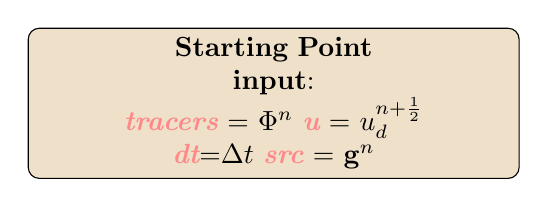
\begin{tikzpicture}
    \node [block](init){
        \textbf{Starting Point}\\
        \textbf{input}: \\
        \para{tracers} = $\Phi^n$ \para{u} = $u_d^{n+ \frac{1}{2}}$\\ \para{dt}=$\Delta t$ \para{src} = $ \mathbf{g}^n$\\
      };
  \end{tikzpicture}
  \columnbreak
  \begin{minted}[obeytabs=false,mathescape=true,breaklines]{lexer.py:DiffLexer -x}
    struct Advection {
      scalar * tracers;
      face vector u;
      double dt;
      scalar * src; // optional
    };
    void advection (struct Advection p)
    {
      scalar * lsrc = p.src;
      if (!lsrc)
        for (scalar s in p.tracers)
          lsrc = list_append (lsrc, zeroc);
      assert (list_len(p.tracers) == list_len(lsrc));
  \end{minted}
\end{multicols}

\begin{center}
  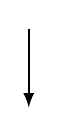
\begin{tikzpicture}
    \draw[-latex,thick](0,0) -- (0,-1); 
  \end{tikzpicture}
\end{center}

\begin{multicols}{2}
  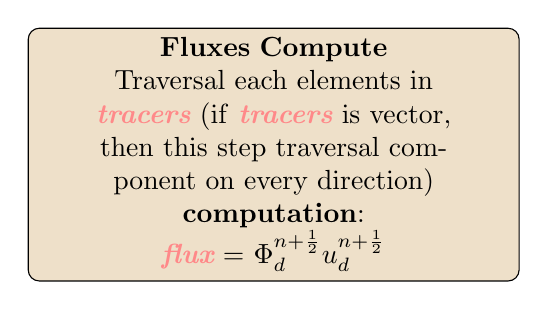
\begin{tikzpicture}
    \node [block](init){
        \textbf{Fluxes Compute}\\
        Traversal each elements in \para{tracers} (if \para{tracers} is vector, then this step traversal component on every direction)\\
        \textbf{computation}: \\
        \para{flux} = $\Phi^{n+ \frac{1}{2}}_d u_d^{n+ \frac{1}{2}}$\\
      };
  \end{tikzpicture}
  \columnbreak
  \begin{minted}[obeytabs=false,mathescape=true,breaklines]{lexer.py:DiffLexer -x}
  scalar f, src;
  for (f,src in p.tracers,lsrc) {
    face vector flux[];
    tracer_fluxes (f, p.u, flux, p.dt, src);
  \end{minted}
\end{multicols}

\begin{center}
  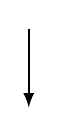
\begin{tikzpicture}
    \draw[-latex,thick](0,0) -- (0,-1); 
  \end{tikzpicture}
\end{center}


\begin{multicols}{2}
  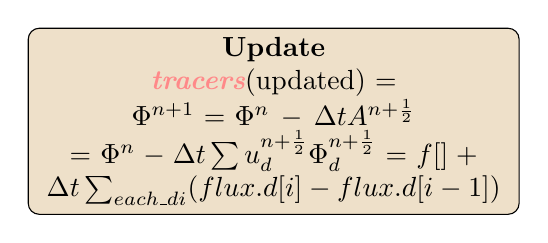
\begin{tikzpicture}
    \node [block](init){
        \textbf{Update}\\
        \para{tracers}(updated) = $\Phi^{n+1}$ = $\Phi^n-\Delta t A^{n+ \frac{1}{2}}$\\
        = $\Phi^n- \Delta t \sum u_d^{n+ \frac{1}{2}}\Phi_d^{n + \frac{1}{2}}$
        = $f[] + \Delta t \sum_{each\_di} (flux.d[i]-flux.d[i-1])$
      };
  \end{tikzpicture}
  \columnbreak
  \begin{minted}[obeytabs=false,mathescape=true,breaklines]{lexer.py:DiffLexer -x}
    #if !EMBED
        foreach()
          foreach_dimension()
            f[] += p.dt*(flux.x[] - flux.x[1])/(Delta*cm[]);
    #else // EMBED
        update_tracer (f, p.u, flux, p.dt);//This is a function that induced by embed.h which conducts same procedure with special care taken for embed boundary.
    #endif // EMBED
      }

      if (!p.src)
        free (lsrc);
    }
  \end{minted}
\end{multicols}

\appendix
\section{Caculation of Face Centered Normal Veloctiy}
It can be seen from \ref{sec:intro}, the computation of face centered normal velocity $u_d^{n+ \frac{1}{2}}$ is of great importance to construct advection term. The detailed procedure of extrapolation is shown in documentation of \textbf{cnetered.h}. The output of such variable follows a similiar step as Eq.\ref{equ:taylor} but without pressure term since the face centered velocity will be projected with an edge-centered projection. This additional projection ensures the feature of conservative of corresponding method.\par
When it comes to the resolution of NS equation, $\Phi$ in governing eqaution \ref{equ:aim} is the cell-centered vector $ \mathbf{u}^n$. According to Martin\cite{martin2000cell}, normal components caculated by Eq.\ref{equ:taylor} can simply be replaced by $u_d^{n+ \frac{1}{2}}$, which means we only need to compute tangential fluxes. However, after series of tests, reuse of normal fluxes will lead to unstable at sharp angles. Thus all components is recomputed in Basilisk\cite{popinet2003gerris}.
\printbibliography
\end{document}
